% !TeX root = ../main.tex

\begin{frame}
  \begin{textblock*}{11cm}(0cm,1cm)
    \begin{small}
    \begin{description}
      \item[Goal:] Show $\ell : \hom_0(\overline{B_\omega}, \overline{D})\to \hom_0(\overline{Q^\delta},\overline{P^\delta})$ is injective

      \item[Method:] Check
      % \only<1>{Check $\mathbf{dim}~\hom_0(D\setminus B_\omega)\leq \mathbf{dim}~\hom_0(\overline{Q^\delta}, \overline{P^\delta})$.}
      \[  \only<1-2>{\mathbf{rk}~\hom_0((\overline{Q_1^\delta}, \overline{P^\delta})\hookrightarrow (\overline{Q_0^\delta}, \overline{P^\delta}))\geq {\color<2>{red}\mathbf{dim}~\hom_0(D\setminus B_\omega)}}
          \only<3-4>{{\color<4>{red}\mathbf{rk}~\hom_0((\overline{Q_1^\delta}, \overline{P^\delta})\hookrightarrow (\overline{Q_0^\delta}, \overline{P^\delta}))}\geq \mathbf{dim}~\hom_0(\rips^\delta(P\setminus Q_{0}))}.\]
      % \item[Method:] Check $\mathbf{dim}~\hom_0(D\setminus B_\omega)\leq \mathbf{dim}~\hom_0(\overline{Q^\delta}, \overline{P^\delta})$
      \item[Problems:]
    \end{description}
    \end{small}
  \end{textblock*}

  \begin{textblock*}{11cm}(1cm,4.75cm)
    \begin{small}
    \begin{enumerate}[a]
      \item $\mathbf{dim}~\hom_0(\overline{Q^\delta}, \overline{P^\delta})\geq \mathbf{dim}~\hom_0(D\setminus B_\omega)\nRightarrow \ell$ injective,
      \item $\mathbf{dim}~\hom_0(D\setminus B_\omega)$ unknown
      \item Cannot compute homology groups of complements
      \item Cannot compute homology of offsets
    \end{enumerate}
    \end{small}
  \end{textblock*}
\end{frame}

\begin{frame}
  \frametitle{Duality}

  \begin{textblock*}{11cm}(1cm,2cm)
    \begin{small}
      \begin{enumerate}[a]
        \setcounter{enumi}{2}
        \item Cannot compute homology groups of complements
        % \item Cannot compute homology of offsets
      \end{enumerate}%\vspace{1ex}
    \end{small}

    \only<2-4>{\[\hom_d(P^\e,Q^\e)\cong\hom_0(D\setminus Q^\e, D\setminus P^\e).\]}
  \end{textblock*}

  \begin{textblock*}{11cm}(1cm,5.5cm)
    \centering
    \includegraphics<2>[width=0.8\textwidth]{figures/balloons1}%
    \includegraphics<3>[width=0.8\textwidth]{figures/balloons2}%
    \includegraphics<4>[width=0.8\textwidth]{figures/balloons3}
  \end{textblock*}
\end{frame}

\begin{frame}
  \frametitle{Duality}

  \begin{textblock*}{11cm}(1cm,2cm)
    \begin{small}
      $\mathbf{rk}~\hom_0((\overline{Q_1^\delta}, \overline{P^\delta})\hookrightarrow(\overline{Q_1^\delta}, \overline{P^\delta})) = \mathbf{rk}~\hom_d((P^\delta, Q_0^\delta)\hookrightarrow (P^\delta, Q_1^\delta))$

      % \only<3>{Check $\mathbf{rk}~\hom_d((P^\delta, Q_0^\delta)\hookrightarrow (P^\delta, Q_1^\delta)) \geq \mathbf{dim}~\hom_0(D\setminus B_\omega)$}
      % \only<4>{Check $\mathbf{rk}~\hom_d((P^\delta, Q_0^\delta)\hookrightarrow (P^\delta, Q_1^\delta)) \geq \mathbf{dim}~\hom_0(\rips^\delta(P\setminus Q_{0}))$}
    \end{small}
  \end{textblock*}

  \begin{textblock*}{6cm}(1cm,4cm)
    \centering
    \includegraphics<1>[trim=50 250 50 300, clip, width=0.5\textwidth]{figures/ass1_2/PQ2comp}%
    \includegraphics<2>[trim=50 250 50 300, clip, width=0.5\textwidth]{figures/ass1_2/PQ2comp-spread}%
  \end{textblock*}
  \begin{textblock*}{6cm}(1cm,6.75cm)
    \centering
    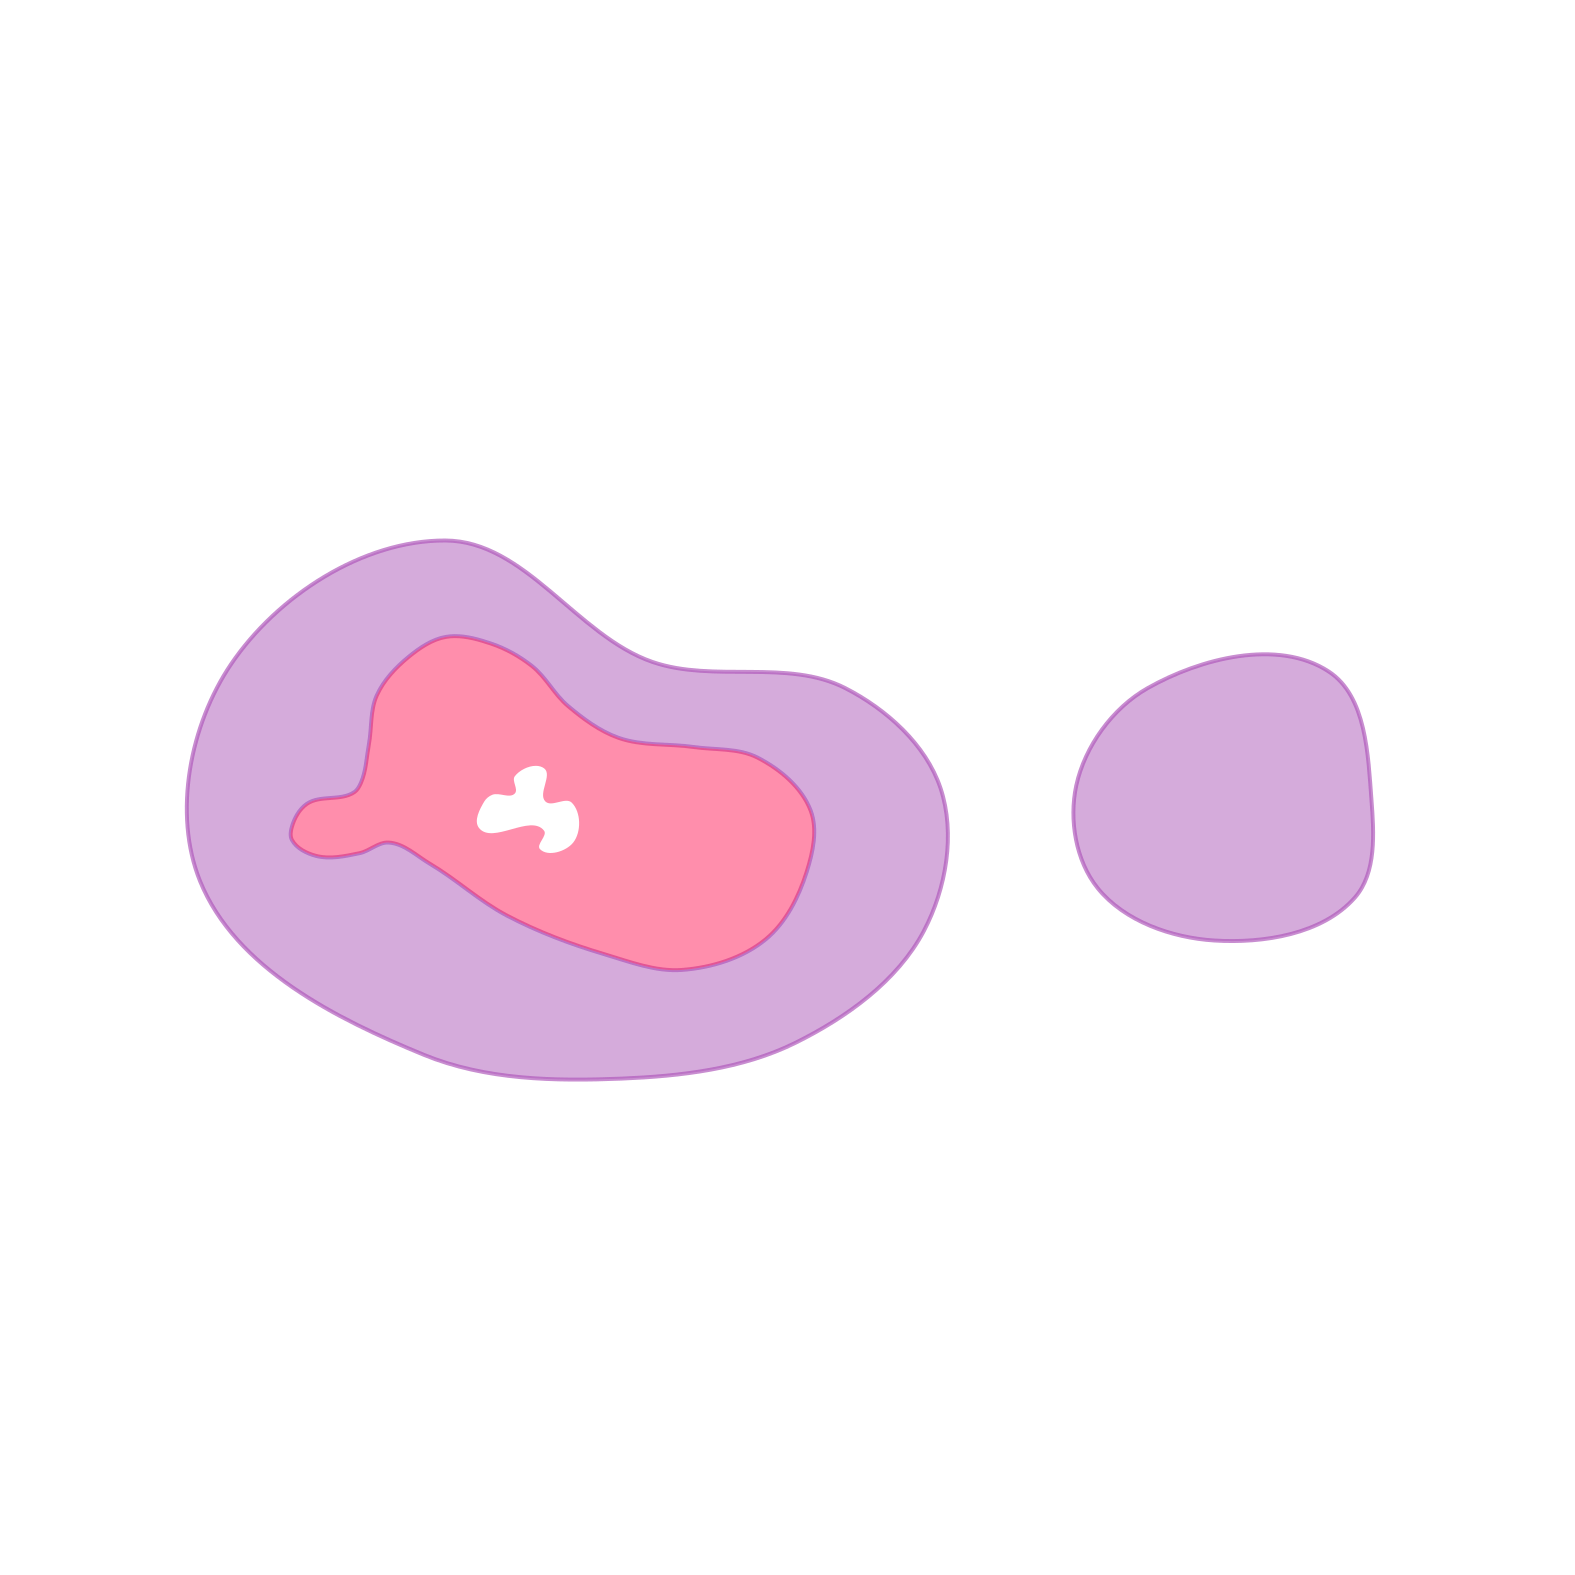
\includegraphics[trim=50 250 50 300, clip, width=0.5\textwidth]{figures/ass1_2/PQ2}%
  \end{textblock*}

  \begin{textblock*}{6cm}(6cm,4cm)
    \centering
    \includegraphics<1>[trim=50 250 50 300, clip, width=0.5\textwidth]{figures/ass1_2/PQ1comp}%
    \includegraphics<2>[trim=50 250 50 300, clip, width=0.5\textwidth]{figures/ass1_2/PQ1comp-spread}%
  \end{textblock*}
  \begin{textblock*}{6cm}(6cm,6.75cm)
    \centering
    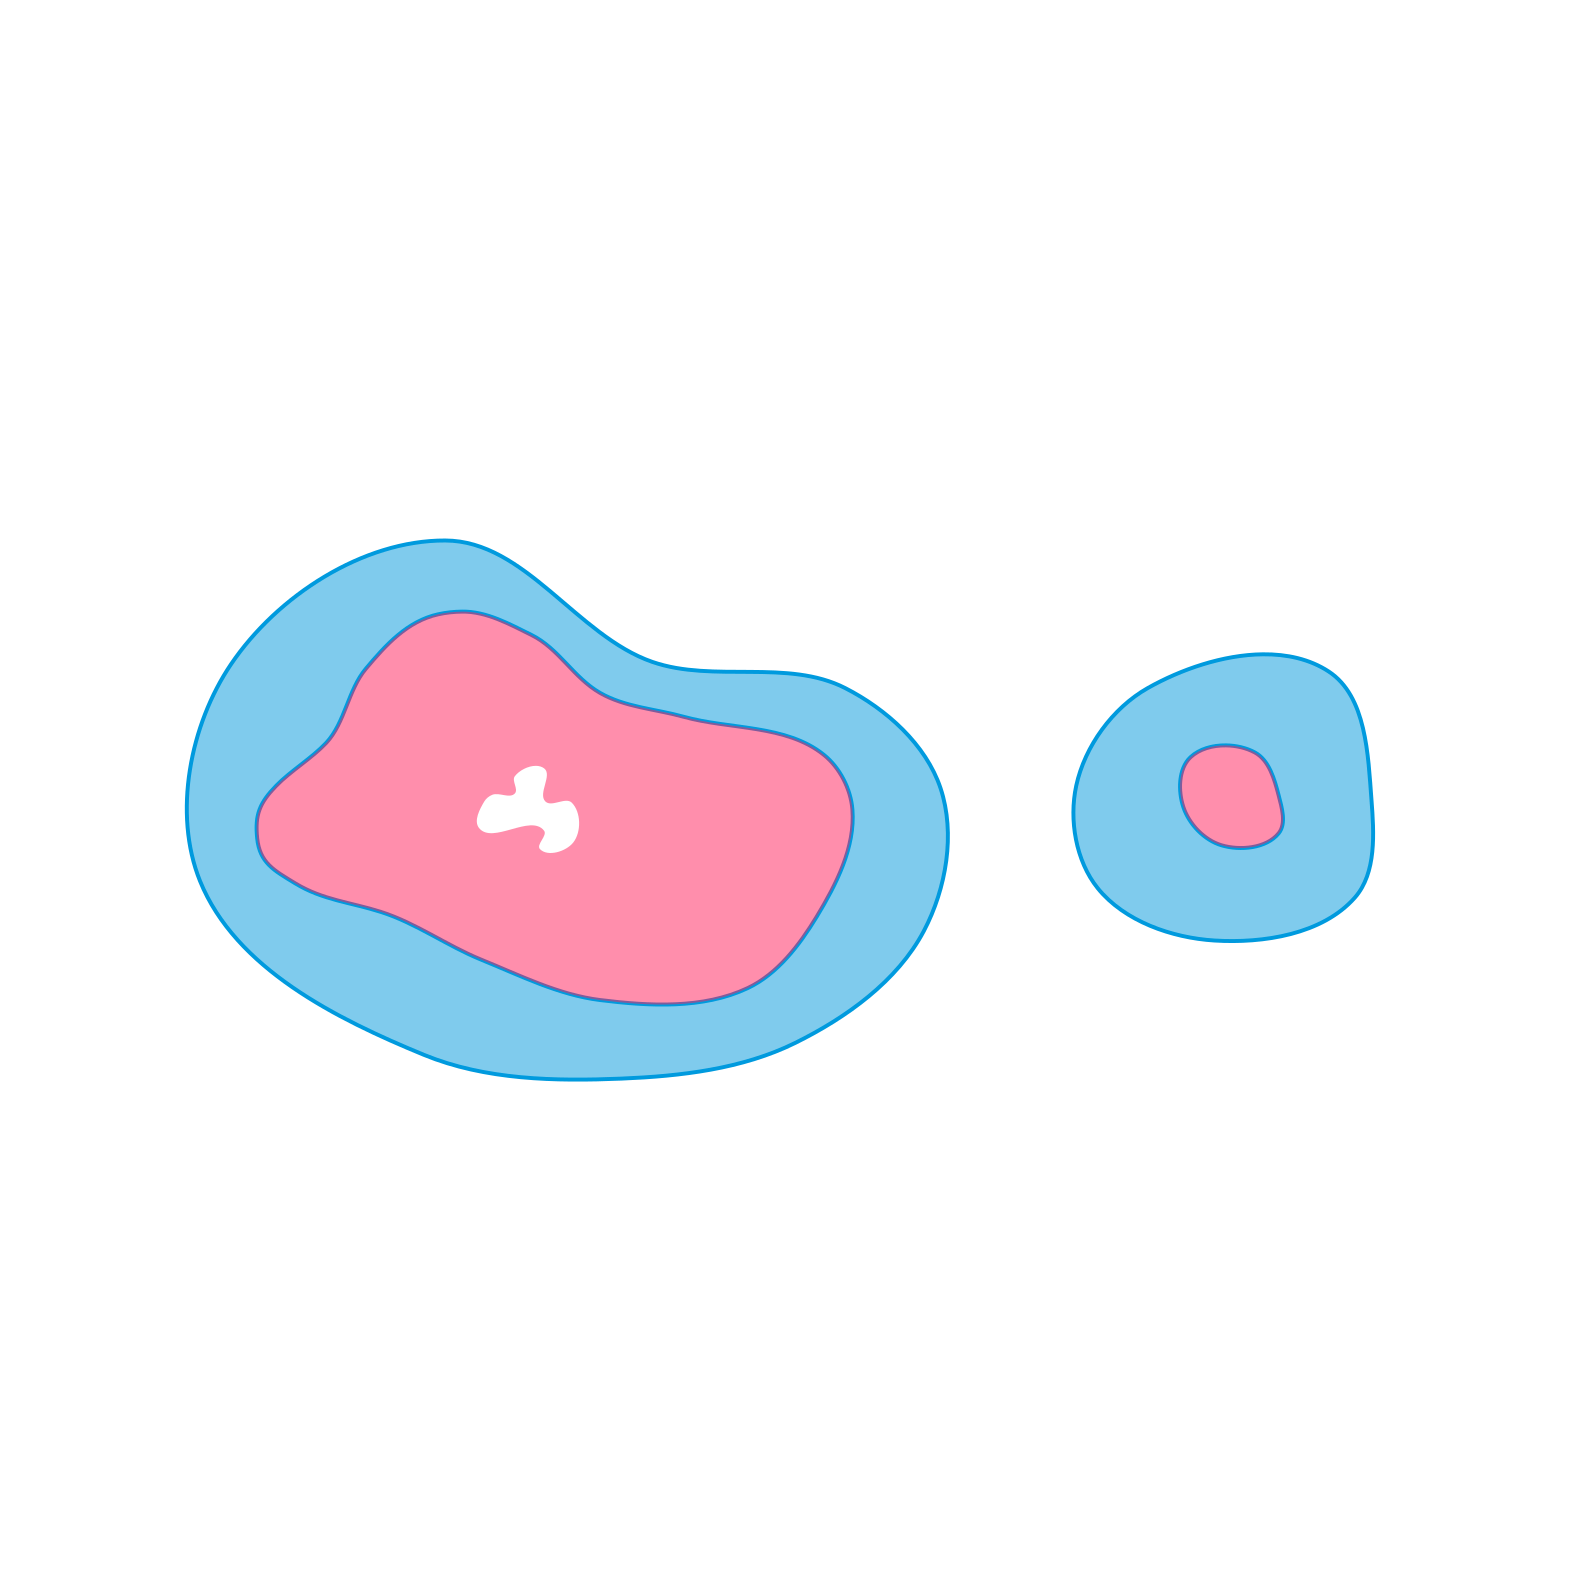
\includegraphics[trim=50 250 50 300, clip, width=0.5\textwidth]{figures/ass1_2/PQ1}%
  \end{textblock*}

\end{frame}
